\chapter{FET in Horizon 2020}
This chapter illustrates the FET initiative and its research lines of relevance for this thesis. Section \ref{The_Horizon_2020_programme} is a concise overview of the Horizon 2020 initiative. Section \ref{The_FET_programme} gives a description of FET in the framework of Horizon 2020 and its main calls for funding. Finally, sections \ref{Quantum_technologies} and \ref{High-performing_computing} summarise the FET effort towards the development of quantum technologies and high-performing computers.

\section{The Horizon 2020 programme} \label{The_Horizon_2020_programme}
Horizon 2020 is the biggest Research and Innovation funding programme financed by the European Union to date. It aims at ensuring a smart and sustainable societal and economic growth by investing on and applying scientific research. The programme has a total budget of nearly 80 billions euro over a seven-year period (from 2014 to 2020).

Horizon 2020 is Europe's eighth Research and Innovation programme in chronological order. Previous programmes were each four years long, with the first launched in 1984. The increasing budget allocated for the Research and Innovation programmes is shown in figure \ref{FP_funds}.

\begin{figure}[!t] 
 \begin{center}
 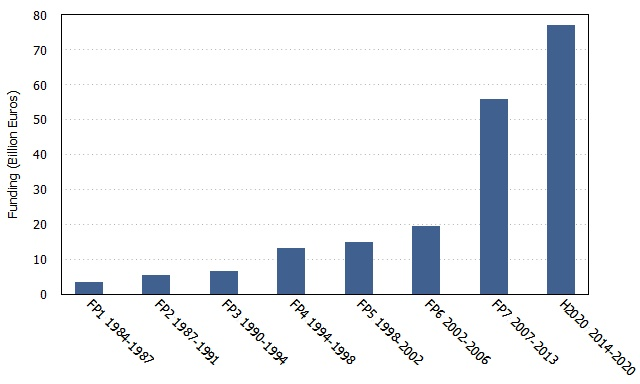
\includegraphics[scale=0.4]{Images/FP_funds.jpg}
 \caption{Budget allocated for Europe's Research and Innovation programmes in billion euros over the past years. FP stands for Framework Programme. Data from \cite{OECD}.}
 \label{FP_funds}
 \end{center}
\end{figure}

%data from https://ec.europa.eu/research/fp7/pdf/fp-1984-2013_en.pdf#view=fit&pagemode=none

Any natural or legal persons such as universities, research organisation, companies etc. can apply for funding from Horizon 2020. Applications must fit into one of the following categories: 

\begin{itemize}
 \item \textbf{Excellent Science:} the goal of this initiative is to support and increase the excellence of European scientific research on a global level in a variety of fields.
 \item \textbf{Industrial Leadership:} this class of projects targets the development of the technological innovations of tomorrow's market and the growth of European small and medium enterprises.
 \item \textbf{Societal Challenges:} this group focuses on priorities of the European society such as health, education, energy supply and food by combining knowledge and methods from different scientific fields and humanities.  
 \item \textbf{European Institute for Innovation and Technology (EIT):} the EIT is an independent European body supporting European growth by promoting synergies among three key societal players: education, research and business. 
 \item \textbf{Euratom:} this pillar focuses on nuclear research and safety with to the goal to contribute to the decarbonisation of the energy supply.
\end{itemize}

The budget breakdown of the Horizon 2020 into the aforementioned lines of action is shown in figure \ref{H2020_budget_breakdown}

\begin{figure}[!t] 
 \begin{center}
 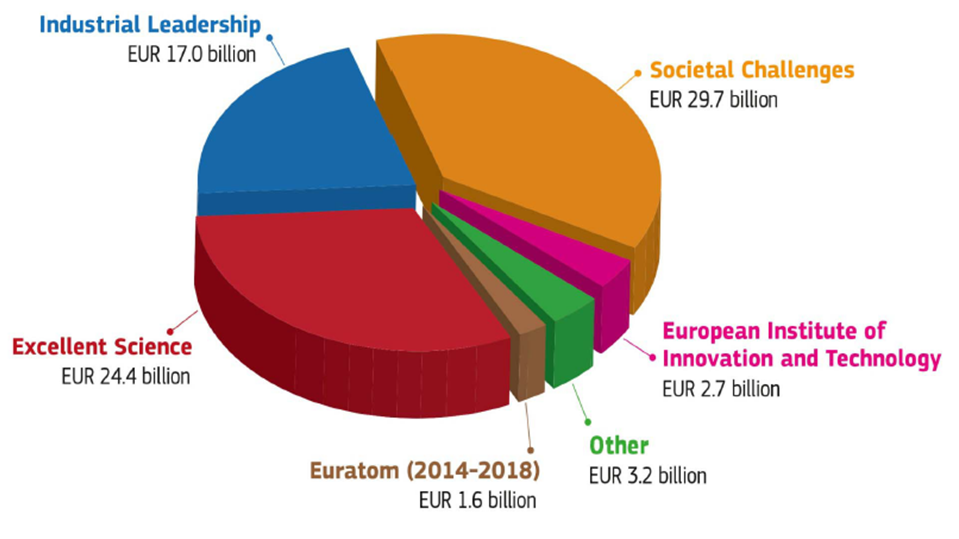
\includegraphics[scale=0.3]{Images/H2020_budget_breakdown.png}
 \caption{Budget breakdown of the Horizon 2020 programme. Original image in \cite{OECD}.}
 \label{H2020_budget_breakdown}
 \end{center}
\end{figure}

\section{The FET programme} \label{The_FET_programme}
As mentioned in section \ref{The_Horizon_2020_programme}, one of the pillars of Horizon 2020 is the Excellent Science programme. This initiative supports researchers and institutions developing new science and cutting-edge technology. The goal is to keep European research at the forefront of scientific innovation and discover applications to improve the citizens' life and ensure economical growth.  

\begin{table}[t]
 \begin{center}
  \begin{tabular}{cc}
   \hline 
   \hline
   Line of action & Estimated final amount \\ 
   \hline
   \hline
   ERC & 13095 \\
   FET & 2696 \\
   MSCA & 6162 \\
   RI & 2488 \\
   \hline
   \hline
  \end{tabular}
 \end{center} 
 \caption{Estimated final budget breakdown of the Excellent Science initiative. ERC stands for European Research Council; FET for Future and Emerging Technologies; MSCA for Marie Sk\l{}odowska-Curie Actions; RI for Research infrastructure. The estimated final amounts are expressed in million euros.}
\label{FET_budget_breakdown} 
\end{table}

Excellent Science is based on the four following pillars: 

\begin{itemize}
 \item \textbf{European Research Council (ERC):} The ERC assigns funding in every field of research to single scientists working in only one host institution and with the requirement of scientific excellence.  
 \item \textbf{Future and Emerging Technologies (FET):} the FET programme finances collaborative research exploring visionary and radically new investigation lines. 
 \item \textbf{Marie Sk\l{}odowska-Curie Actions:} this initiative provides grants for researchers at any stage of their career with the goal to encourage mobility between countries and fields of expertise. 
 \item \textbf{Research infrastructure:} this pillar promotes the creation of networks of transnational research infrastructures as well as the training of qualified staff. 
\end{itemize}

The estimated final budget breakdown of Excellent Science is reported in table \ref{FET_budget_breakdown}.

\begin{figure}[!t] 
 \begin{center}
 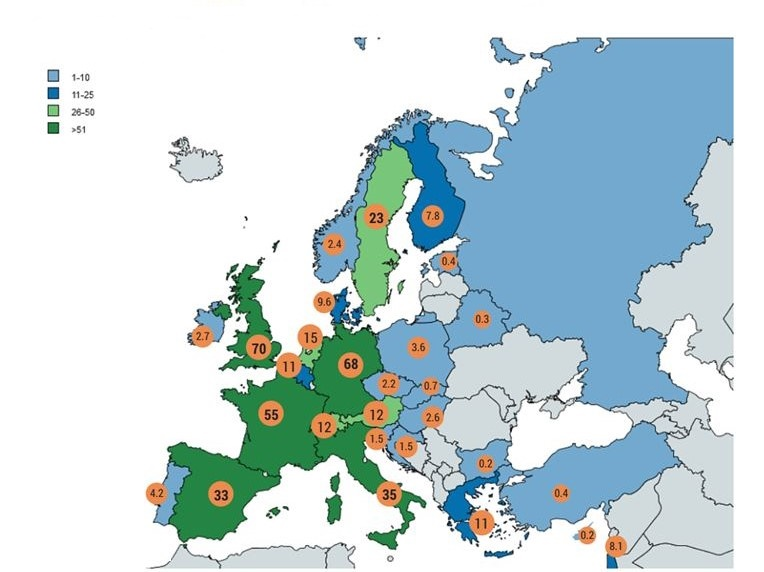
\includegraphics[scale=0.3]{Images/Country_participation_in_H2020_FET_projects.jpg}
 \caption{Participation in the Horizon 2020 FET programme on a country basis as of June 2016. The numbers correspond to FET funding in millions of euro. The colour indicates the number of participants. Adapted from image in ....}
 \label{Country_participation_in_H2020_FET_projects}
 \end{center}
\end{figure}

%image downloaded from https://ec.europa.eu/programmes/horizon2020/en/news/infographic-participation-horizon-2020-fet-projects

The present thesis focuses on the communication activity of the 151 Horizon 2020 projects funded within the FET scheme to date. The complete list of these projects is available in Appendix ... . Their distribution per country as of June 2016 is shown in figure \ref{Country_participation_in_H2020_FET_projects}

The FET funding scheme comprises three calls for applications: FET Open, FET Proactive and FET Flagship.

\subsubsection{FET Open}
The FET Open call is not related to a specific investigation theme. However, submitted research proposals must satisfy the following ``gatekeepers": scientific and technological breakthrough; foundational; novelty; high-risk; long-term vision; interdisciplinary. FET Open promotes the so-called Coordination and Support Actions (CSA) as well. These actions aim at identifying and fulfil the optimal conditions for FET-related collaborative. One CSA type of action is FET Innovation Launchpad, which investigates and explores possible economical and societal applications of results from FET projects.

\subsubsection{FET Proactive}
The FET Proactive call targets the creation of scientific synergies of researchers from 

supports the aims at bringing 

to nurture investigation networks of scientists from interdisciplinary fields by bringing scientists from disparate fields together  of scientists from disparate interdisciplenary fields working together on given topics. The topics are not ready for the market. Currently, FET Proactive comprises three calls related to the topic "Boosting emerging technologies" and three under the topic "High Performance Computing". Given its relevance for the scope of this thesi, the "High Performance Computing" FET PRoactive call is more extensively outlined in section..... Besides this, FET Proactive invests resources also on identifying investigation roadmaps for the considered areas, design and distribute material for educational purposes and disseminate FET results among stakeholders.  

\subsubsection{FET Flagships}
FET Flagships are the main efforts of European research. They are large-scale, decade-long projects each with available budget totalling one billion Euros. The ultimate goals are to shed light on key scientific themes and apply scientific achievements to European society. To date, three FET Flagships have been approved in the Horizon 2020 programme: 

\begin{itemize}
 \item the Human Brain Project, which targets significant step forwards in neuroscience.
 \item Graphene, which exploring Graphene's properties and possible applications.
 \item Quantum technologies, aiming at development of groundbreaking technologies based on the laws of quantum physics.
\end{itemize}
The Human Brain Project and Graphene Flagship started in April 2016. The Quantum technologies Flagship will start running in 2018. Given the importance for the scope of this thesis, the Quantum technologies flaghisp is described in more detail in section ...

\section{Quantum technologies} \label{Quantum_technologies}
Quantum technologies arise from applications of quantum physics. They are an important research topic on a global level for their potential to revolutionise human societies.

The so-called first quantum revolution started at the beginning of the past century with the development of quantum theory. The growing understanding of the world on the atomic scale led to the birth of new disciplines such as informatics and microelectronics and to the construction of countless fundamental tools and electronic devices. Examples range from computers and cameras to lasers and photocopy machines. The first quantum revolution played a key role in opening the knowledge era of human society.

It is believed that the second quantum revolution will be driven by the ability acquired by humankind to actively engineer the quantum world to its own purposes. This is expected to lead to a complete new class of technologies capable of revolutionise key aspects of our society such as communication and security. The main goal of the second quantum revolution is the development of quantum computers. If successfully developed, such machines will be far more powerful than any present and future computer based on classical architectures. The urge for Europe to stay at the forefront of the second quantum revolution is outlined in the so-called Quantum Manifesto.

%citazione articolo arxiv https://arxiv.org/ftp/quant-ph/papers/0206/0206091.pdf

The development of quantum technologies is a central objective of the FET programme. As mentioned in section \ref{The_FET_programme}, one flagship initiative in this investigation area will be launched next year. Moreover, a number of FET research projects in the field of quantum technologies is already running. The list of Horizon 2020 FET projects in this field is reported in Appendix ... . Their activity is supported by the ERANET Cofund in Quantum Technologies, a FET Proactive initiative aiming the creation of synergies and partnerships among researchers and disparate kinds of stakeholders. 

\section{High-performing computing} \label{High-performing_computing}
Current and future scientific and engineering challenges demand increasing levels of computational performances. This is targeted through the construction of large computer clusters and the development of suitable programming languages. The former provide higher computational power, the latter an optimal exploitation of the clusters' resources. The use of such practices is known as high-performing computing (HPC).

In terms of increasing computational power, one major HPC goal is the transition from the peta- to the exascale. This corresponds to the increase from $10^{15}$ floating point operations per second, the limit of today's most powerful supercomputers, to $10^{18}$. The upgrade to the exascale is believed to have a major impact in practice all fields of science, driving research and the development of new technology in the next decades. 

European HPC effort is funded within the FET Proactive call ``High Performance Computing". This call comprises three initiatives: \textit{i}) co-design of HPC systems and applications; \textit{ii}) transition to exascale computing; and \textit{iii}) exascale HPC ecosystem development. The main goals of the three initiatives are the development of next-generation high-performing computers towards exascale and providing access to the resources offered by supercomputers. The list of Horizon 2020 FET projects active in the field of HPC and transition to the exascale is available in Appendix ... .

\section{Chapter summary} 
In this chapter, the following items have been discussed:

\begin{enumerate}
 \item Horizon 2020 is the largest research funding programme of the European Union. It is planned to run from 2014 to 2020 and has a total budget of nearly 80 billion Euros. 
 \item One of Horizon 2020's funding schemes is Future and Emerging Technologies (FET). The FET call finances visionary research projects targeting scientific breakthroughs and the development and application of radically new technologies. The estimated FET final budget will total nearly 3 billion Euros. 
 \item The development of quantum technologies is part of the FET effort. In particular, a FET Flagship on quantum technologies has been approved in 2016 by the European Commission and will start in 2018. Allocated funds sum up to one billion Euros. 
 \item Another major goal of the FET initiative is the development of high-performing computers. The main focus of this investigation line is a power increase of three orders of magnitude in modern supercomputers (from $10^{15}$ to $10^{18}$ floating point operations per second). The upgrade from peta- to exascale will provide the scientific community with unprecedented computational resources in practically all fields.    
\end{enumerate}